\chapter{Metaphors for Bitcoin's Future}
\label{les:21}

\begin{chapquote}{Lewis Carroll, \textit{Alice in Wonderland}}
\enquote{I know something interesting is sure to happen\ldots}
\end{chapquote}

In the last couple of decades, it became apparent that technological
innovation does not follow a linear trend. Whether you believe in the
technological singularity or not, it is undeniable that progress is
exponential in many fields. Not only that, but the rate at which
technologies are being adopted is accelerating, and before you know it
the bush in the local schoolyard is gone and your kids are using
Snapchat instead. Exponential curves have the tendency to slap you in
the face way before you see them coming.

Bitcoin is an exponential technology built upon exponential technologies.
\textit{Our World in Data}\footnote{\url{https://ourworldindata.org/}}
beautifully shows the rising speed of technological adoption, starting in 1903
with the introduction of landlines (see Figure~\ref{fig:tech-adoption}).
Landlines, electricity, computers, the internet, smartphones; all follow
exponential trends in price-performance and adoption. Bitcoin does
too~\cite{tech-adoption}.

\begin{center}
  \includegraphics[width=\textwidth]{assets/images/tech-adoption.png}
  \caption{Bitcoin is literally off the charts.}
  \label{fig:tech-adoption}
\end{center}

Bitcoin has not one but multiple network effects\footnote{Trace Mayer,
\textit{The Seven Network Effects of Bitcoin}~\cite{7-network-effects}}, all of
which resulting in exponential growth patterns in their respective area: price,
users, security, developers, market share, and adoption as global money.

Having survived its infancy, Bitcoin is continuing to grow every day in
more aspects than one. Granted, the technology has not reached maturity
yet. It might be in its adolescence. But if the technology is
exponential, the path from obscurity to ubiquity is short.

\begin{center}
  \includegraphics[width=\textwidth]{assets/images/mobile-phone.png}
  \caption{Mobile phone, ca 1965 vs 2019.}
  \label{fig:mobile-phone}
\end{center}

In his 2003 TED talk, Jeff Bezos chose to use electricity as a metaphor for the
web's future.\footnote{\url{http://bit.ly/bezos-web}} All three phenomena ---
electricity, the internet, Bitcoin --- are \textit{enabling} technologies,
networks which enable other things. They are infrastructure to be built upon,
foundational in nature.

Electricity has been around for a while now. We take it for granted. The
internet is quite a bit younger, but most people already take it for
granted as well. Bitcoin is ten years old and has entered public
consciousness during the last hype cycle. Only the earliest of adopters
take it for granted. As more time passes, more and more people will
recognize Bitcoin as something which simply is.\footnote{This is known as the
\textit{Lindy Effect}. The Lindy effect is a theory that the future life expectancy
of some non-perishable things like a technology or an idea is proportional to
their current age, so that every additional period of survival implies a longer
remaining life expectancy.~\cite{wiki:lindy}}

In 1994, the internet was still confusing and unintuitive. Watching this old
recording of the \textit{Today
Show}\footnote{\url{https://youtu.be/UlJku_CSyNg}} makes it obvious that what
feels natural and intuitive now actually wasn't back then. Bitcoin is still
confusing and alien to most, but just like the internet is second nature for
digital natives, spending and stacking
sats\footnote{\url{https://twitter.com/hashtag/stackingsats}} will be second
nature to the bitcoin natives of the future.

\begin{quotation}\begin{samepage}
\enquote{The future is already here --- it's just not very evenly
distributed.}
\begin{flushright} -- William Gibson\footnote{William Gibson, \textit{The Science in Science Fiction} \cite{william-gibson}}
\end{flushright}\end{samepage}\end{quotation}

In 1995, about $15\%$ of American adults used the internet. Historical
data from the Pew Research Center~\cite{pew-research} shows how the internet has woven
itself into all our lives. According to a consumer survey by Kaspersky
Lab~\cite{web:kaspersky}, 13\% of respondents have used Bitcoin and its clones to pay for
goods in 2018. While payments aren't the only use-case of bitcoin, it is
some indication of where we are in Internet time: in the early- to
mid-90s.

In 1997, Jeff Bezos stated in a letter to shareholders~\cite{bezos-letter} that
\enquote{this is Day 1 for the Internet,} recognizing the great untapped
potential for the internet and, by extension, his company. Whatever day this is
for Bitcoin, the vast amounts of untapped potential are clear to all but the
most casual observer.

\begin{center}
  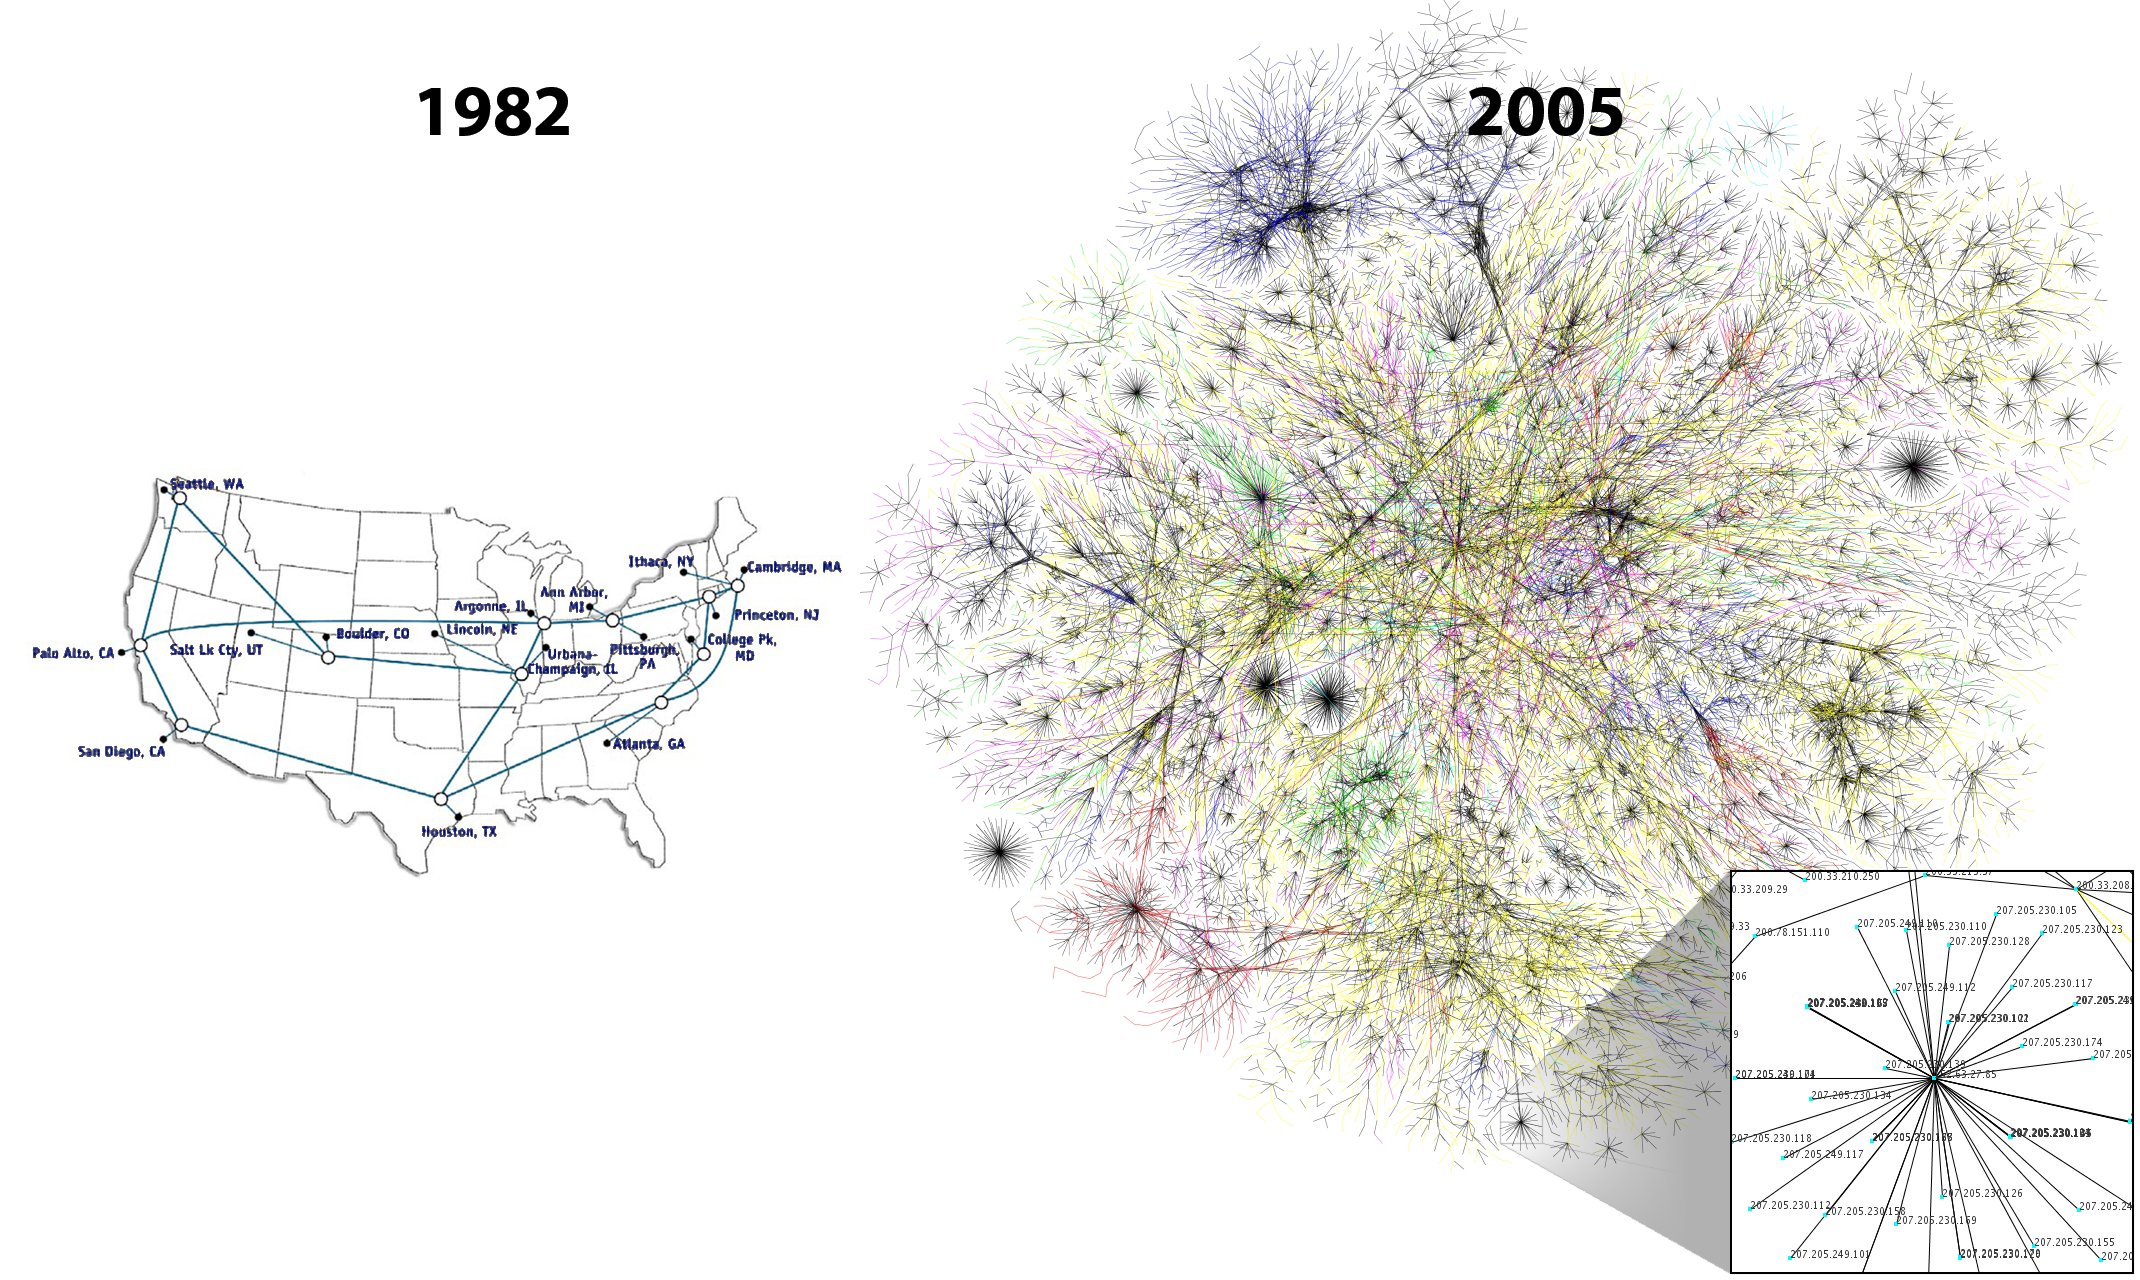
\includegraphics[width=\textwidth]{assets/images/internet-evolution-white-dates.png}
  \caption{The internet, 1982 vs 2005. Source: cc-by Merit Network, Inc. and Barrett Lyon, Opte Project}
  \label{fig:internet-evolution-white-dates}
\end{center}

Bitcoin's first node went online in 2009 after Satoshi mined the \textit{genesis
block}\footnote{The genesis block is the first block of the Bitcoin block chain.
Modern versions of Bitcoin number it as block $0$, though very early versions
counted it as block $1$. The genesis block is usually hardcoded into the
software of the applications that utilize the Bitcoin block chain. It is a
special case in that it does not reference a previous block and produces an
unspendable subsidy. The \textit{coinbase} parameter contains, along with the
normal data, the following text: \textit{\enquote{The Times 03/Jan/2009 Chancellor on
brink of second bailout for banks}} \cite{btcwiki:genesis-block}} and released
the software into the wild. His node wasn't alone for long. Hal Finney was one
of the first people to pick up on the idea and join the network. Ten years
later, as of this writing, more than
$75.000$\footnote{\url{https://bit.ly/luke-nodecount}} nodes are running
bitcoin.

\begin{center}
  \centering
  \includegraphics[width=8cm]{assets/images/running-bitcoin.png}
  \caption{Hal Finney authored the first tweet mentioning bitcoin in January 2009.}
  \label{fig:running-bitcoin}
\end{center}

The protocol's base layer isn't the only thing growing exponentially.
The lightning network, a second layer technology, is growing at an even
faster rate.

In January 2018, the lightning network had $40$ nodes and $60$
channels~\cite{web:lightning-nodes}. In April 2019, the network grew to more
than $4000$ nodes and around $40.000$ channels. Keep in mind that this is still
experimental technology where loss of funds can and does occur. Yet the trend is
clear: thousands of people are reckless and eager to use it.

\begin{center}
  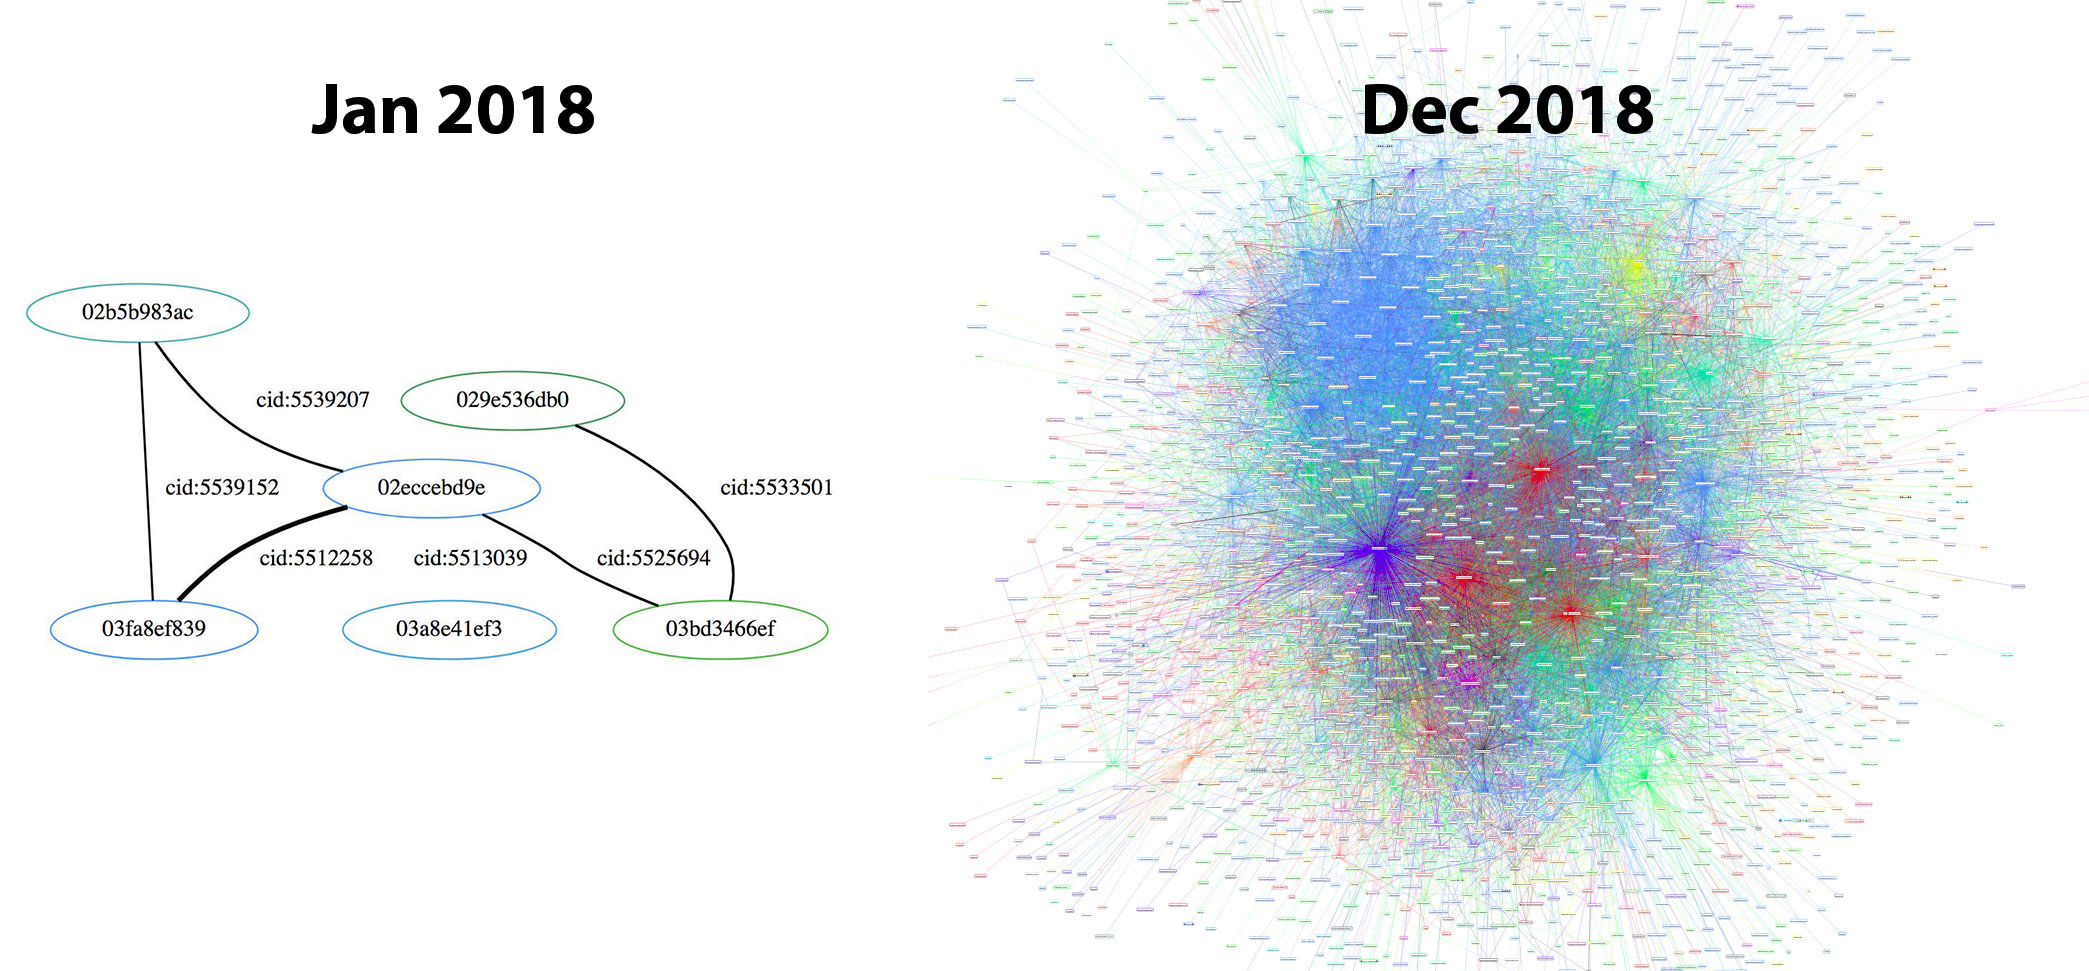
\includegraphics[width=\textwidth]{assets/images/lnd-growth-lopp-white.png}
  \caption{Lightning Network, January 2018 vs December 2018. Source: Jameson Lopp}
  \label{fig:lnd-growth-lopp-white.png}
\end{center}

To me, having lived through the meteoric rise of the web, the parallels
between the internet and Bitcoin are obvious. Both are networks, both
are exponential technologies, and both enable new possibilities, new
industries, new ways of life. Just like electricity was the best
metaphor to understand where the internet is heading, the internet might
be the best metaphor to understand where bitcoin is heading. Or, in the
words of Andreas Antonopoulos, Bitcoin is \textit{The Internet of Money}.
These metaphors are a great reminder that while history doesn't repeat
itself, it often rhymes.

Exponential technologies are hard to grasp and often underestimated.
Even though I have a great interest in such technologies, I am
constantly surprised by the pace of progress and innovation. Watching
the Bitcoin ecosystem grow is like watching the rise of the internet in
fast-forward. It is exhilarating.

My quest of trying to make sense of Bitcoin has led me down the pathways
of history in more ways than one. Understanding ancient societal
structures, past monies, and how communication networks evolved were all
part of the journey. From the handaxe to the smartphone, technology has
undoubtedly changed our world many times over. Networked technologies
are especially transformational: writing, roads, electricity, the
internet. All of them changed the world. Bitcoin has changed mine and
will continue to change the minds and hearts of those who dare to use
it.

\paragraph{Bitcoin taught me that understanding the past is essential to
understanding its future. A future which is just beginning\ldots}

% ---
%
% #### Down the Rabbit Hole
%
% - [The Rising Speed of Technological Adoption][the rising speed of technological adoption] by Jeff Desjardins
% - [The 7 Network Effects of Bitcoin][multiple network effects] by Trace Mayer
% - [The Electricity Metaphor for the Web's Future][TED talk] by Jeff Bezos
% - [How the internet has woven itself into American life][data from the Pew Research Center] by Susannah Fox and Lee Rainie
% - [Genesis Block][genesis block] on the Bitcoin Wiki
% - [Lindy Effect][more time] on Wikipedia
%
% [Our World in Data]: https://ourworldindata.org/
% [the rising speed of technological adoption]: https://www.visualcapitalist.com/rising-speed-technological-adoption/
% [multiple network effects]: https://www.thrivenotes.com/the-7-network-effects-of-bitcoin/
% [TED talk]: https://www.ted.com/talks/jeff_bezos_on_the_next_web_innovation
% [recording of the Today Show]: https://www.youtube.com/watch?v=UlJku_CSyNg
% [William Gibson]: https://www.npr.org/2018/10/22/1067220/the-science-in-science-fiction
% [data from the Pew Research Center]: https://www.pewinternet.org/2014/02/27/part-1-how-the-internet-has-woven-itself-into-american-life/
% [consumer survey]: https://www.kaspersky.com/blog/money-report-2018/
% [letter to shareholders]: http://media.corporate-ir.net/media_files/irol/97/97664/reports/Shareholderletter97.pdf
% [running bitcoin]: https://twitter.com/halfin/status/1110302988?lang=en
% [40 nodes]: https://bitcoinist.com/bitcoin-lightning-network-mainnet-nodes/
% [reckless]: https://twitter.com/hashtag/reckless
% [Jameson Lopp]: https://twitter.com/lopp/status/1077200836072296449
% [\textit{The Internet of Money}]: https://theinternetofmoney.info/
% [stacking]: https://twitter.com/hashtag/stackingsats
%
% <!-- Bitcoin Wiki -->
% [genesis block]: https://en.bitcoin.it/wiki/Genesis_block
%
% <!-- Wikipedia -->
% [more time]: https://en.wikipedia.org/wiki/Lindy_effect
% [alice]: https://en.wikipedia.org/wiki/Alice%27s_Adventures_in_Wonderland
% [carroll]: https://en.wikipedia.org/wiki/Lewis_Carroll
